\documentclass[12pt]{article}
\usepackage[english]{babel}
\usepackage[utf8]{inputenc}
\usepackage{amsmath, amssymb, amsthm}
\usepackage{graphicx}
\usepackage{hyperref}
\usepackage{geometry}
\usepackage{xcolor}
\usepackage{tikz}

\setlength{\topmargin}{0pt}
\setlength{\headsep}{0pt}
\textheight = 600pt

\title{Graph Theory \\ Homework 4}
\author{Ben Kallus and Maddy LaPoint}
\date{Due Monday, February 15}

\begin{document}
\maketitle

\noindent{\bf FIRST}

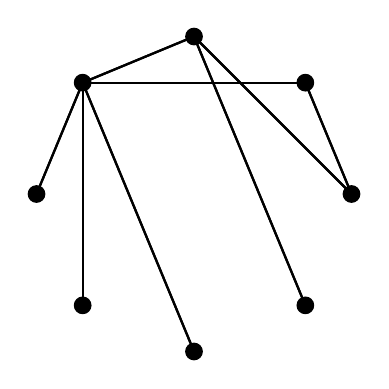
\begin{tikzpicture}
\draw[fill=black] (2.0, 0.0) circle (3pt);
\draw[fill=black] (1.414, 1.414) circle (3pt);
\draw[fill=black] (0.0, 2.0) circle (3pt);
\draw[fill=black] (-1.414, 1.414) circle (3pt);
\draw[fill=black] (-2.0, 0.0) circle (3pt);
\draw[fill=black] (-1.414, -1.414) circle (3pt);
\draw[fill=black] (-0.0, -2.0) circle (3pt);
\draw[fill=black] (1.414, -1.414) circle (3pt);

\draw[thick] (2.0, 0.0) -- (0.0, 2.0);
\draw[thick] (2.0, 0.0) -- (1.414, 1.414);
\draw[thick] (1.414, 1.414) -- (-1.414, 1.414);
\draw[thick] (1.414, 1.414) -- (2.0, 0.0);
\draw[thick] (0.0, 2.0) -- (-1.414, 1.414);
\draw[thick] (0.0, 2.0) -- (1.414, -1.414);
\draw[thick] (0.0, 2.0) -- (2.0, 0.0);
\draw[thick] (-1.414, 1.414) -- (-2.0, 0.0);
\draw[thick] (-1.414, 1.414) -- (-0.0, -2.0);
\draw[thick] (-1.414, 1.414) -- (0.0, 2.0);
\draw[thick] (-1.414, 1.414) -- (1.414, 1.414);
\draw[thick] (-1.414, 1.414) -- (-1.414, -1.414);
\draw[thick] (-2.0, 0.0) -- (-1.414, 1.414);
\draw[thick] (-1.414, -1.414) -- (-1.414, 1.414);
\draw[thick] (-0.0, -2.0) -- (-1.414, 1.414);
\draw[thick] (1.414, -1.414) -- (0.0, 2.0);
\end{tikzpicture}
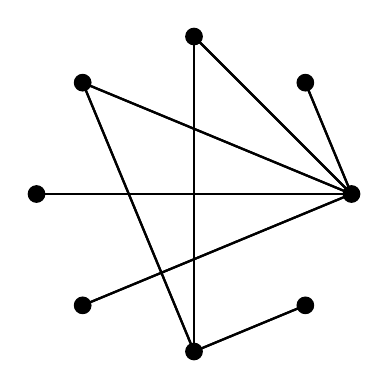
\begin{tikzpicture}
\draw[fill=black] (2.0, 0.0) circle (3pt);
\draw[fill=black] (1.414, 1.414) circle (3pt);
\draw[fill=black] (0.0, 2.0) circle (3pt);
\draw[fill=black] (-1.414, 1.414) circle (3pt);
\draw[fill=black] (-2.0, 0.0) circle (3pt);
\draw[fill=black] (-1.414, -1.414) circle (3pt);
\draw[fill=black] (-0.0, -2.0) circle (3pt);
\draw[fill=black] (1.414, -1.414) circle (3pt);

\draw[thick] (2.0, 0.0) -- (-1.414, 1.414);
\draw[thick] (2.0, 0.0) -- (-1.414, -1.414);
\draw[thick] (2.0, 0.0) -- (1.414, 1.414);
\draw[thick] (2.0, 0.0) -- (0.0, 2.0);
\draw[thick] (2.0, 0.0) -- (-2.0, 0.0);
\draw[thick] (1.414, 1.414) -- (2.0, 0.0);
\draw[thick] (0.0, 2.0) -- (-0.0, -2.0);
\draw[thick] (0.0, 2.0) -- (2.0, 0.0);
\draw[thick] (-1.414, 1.414) -- (-0.0, -2.0);
\draw[thick] (-1.414, 1.414) -- (2.0, 0.0);
\draw[thick] (-2.0, 0.0) -- (2.0, 0.0);
\draw[thick] (-1.414, -1.414) -- (2.0, 0.0);
\draw[thick] (-0.0, -2.0) -- (-1.414, 1.414);
\draw[thick] (-0.0, -2.0) -- (0.0, 2.0);
\draw[thick] (-0.0, -2.0) -- (1.414, -1.414);
\draw[thick] (1.414, -1.414) -- (-0.0, -2.0);
\end{tikzpicture}
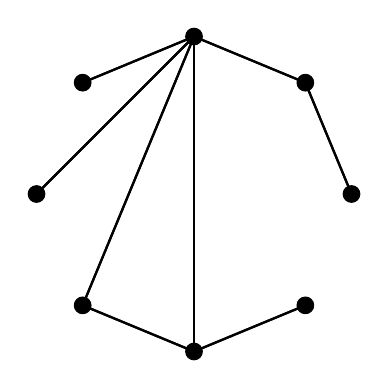
\begin{tikzpicture}
\draw[fill=black] (2.0, 0.0) circle (3pt);
\draw[fill=black] (1.414, 1.414) circle (3pt);
\draw[fill=black] (0.0, 2.0) circle (3pt);
\draw[fill=black] (-1.414, 1.414) circle (3pt);
\draw[fill=black] (-2.0, 0.0) circle (3pt);
\draw[fill=black] (-1.414, -1.414) circle (3pt);
\draw[fill=black] (-0.0, -2.0) circle (3pt);
\draw[fill=black] (1.414, -1.414) circle (3pt);

\draw[thick] (2.0, 0.0) -- (1.414, 1.414);
\draw[thick] (1.414, 1.414) -- (2.0, 0.0);
\draw[thick] (1.414, 1.414) -- (0.0, 2.0);
\draw[thick] (0.0, 2.0) -- (-0.0, -2.0);
\draw[thick] (0.0, 2.0) -- (-1.414, 1.414);
\draw[thick] (0.0, 2.0) -- (-1.414, -1.414);
\draw[thick] (0.0, 2.0) -- (1.414, 1.414);
\draw[thick] (0.0, 2.0) -- (-2.0, 0.0);
\draw[thick] (-1.414, 1.414) -- (0.0, 2.0);
\draw[thick] (-2.0, 0.0) -- (0.0, 2.0);
\draw[thick] (-1.414, -1.414) -- (-0.0, -2.0);
\draw[thick] (-1.414, -1.414) -- (0.0, 2.0);
\draw[thick] (-0.0, -2.0) -- (1.414, -1.414);
\draw[thick] (-0.0, -2.0) -- (-1.414, -1.414);
\draw[thick] (-0.0, -2.0) -- (0.0, 2.0);
\draw[thick] (1.414, -1.414) -- (-0.0, -2.0);
\end{tikzpicture}

\newpage\noindent{\bf 2.31} Proposition: The degree sequence $(d_1, d_2, \hdots, d_n)$ is graphical if and only if the degree sequence $(n-d_n-1, n-d_{n-1}-1, \hdots, n-d_1-1)$ is graphical.
\begin{proof}
    Suppose that the degree sequence $D = (d_1, d_2, \hdots, d_n)$ is graphical.
    Then, there exists a graph $G$ of order $n$ with degree sequence $D$.
    Let $v \in V(G)$.
    Then, $\deg(v) = d_m$, for some $m \in \mathbb N$ satisfying $1 \leq m \leq n$.
    By the definition of $\overline G$, $$\deg_{\overline{G}}(v) + \deg_G(v) = n-1.$$
    Then, $$\deg_{\overline{G}}(v) = n - \deg_G(v) - 1.$$
    Therefore, $$\deg_{\overline{G}}(v) = n - d_m - 1.$$
    Thus, $D' = (n-d_n-1, n-d_{n-1}-1, \hdots, n-d_1-1)$ is the degree sequence for $\overline G$, so $D'$ is graphical.

    Now, suppose that the degree sequence $D' = (n-d_n-1, n-d_{n-1}-1, \hdots, n-d_1-1)$ is graphical.
    Then, by the result of the previous direction of this proof, the degree sequence
    \begin{align*}
        D'' &= (n-(n-d_1-1)-1, n-(n-d_2-1)-1, \hdots, n-(n-d_n-1)-1) \\
            &= (n-n+d_1+1-1, n-n+d_2+1-1, \hdots, n-n+d_n+1-1) \\
            &= (d_1, d_2, \hdots, d_n)
    \end{align*} is graphical.
\end{proof}

\newpage\noindent{\bf 2.32}

\medskip{\bf (a)}
\begin{align*}
    s_1  &= (5,3,3,3,3,2,2,2,1) \\
    s_1' &=   (2,2,2,2,2,2,1,1)
\end{align*}

\medskip{\bf (b)}
\begin{align*}
    s_2  &= (6,3,3,3,3,2,2,2,2,1,1) \\
    s_2' &=   (2,2,2,2,2,2,1,1,1,1)
\end{align*}

\medskip{\bf (c)}
\begin{align*}
    s_3    &= (6,5,5,4,3,2,1) \\
    s_3'   &=   (4,4,3,2,1,0) \\
    s_3''  &=     (3,2,1,0,0)
\end{align*}
$(3,2,1,0,0)$ is not graphical because the presence of a 3 necessitates the existence of at least 4 vertices with nonzero degree.

\medskip{\bf (d)}
\begin{align*}
    s_4   &= (7,5,4,4,4,3,2,1) \\
    s_4'  &=   (4,3,3,3,2,1,0) \\
    s_4'' &=     (2,2,2,1,1,0) % make a new graph for this one.
\end{align*}

\medskip{\bf (e)}
\begin{align*}
    s_5    &= (7,6,5,4,4,3,2,1) \\
    s_5'   &=   (5,4,3,3,2,1,0) \\
    s_5''  &=     (3,2,2,1,0,0) \\
    s_5''' &=       (1,1,0,0,0) % and this one too.
\end{align*}

\bigskip\noindent{\bf 2.36} Proposition: The smallest positive integer $k$ such that the sequence obtained by listing each element of $\{2,6,7\}$ a total of $k$ times is a degree sequence of some graph is 4.
\begin{proof}
    Let $S = \{2,6,7\}$.
    Let $k$ be the smallest positive integer such that the sequence obtained by listing each element of $S$ a total of $k$ times is a degree sequence of some graph.
    Since $7 \in S$, any graph with a degree sequence of the desired form must have at least 8 vertices.
    Thus, $k \cdot |S| \geq 8$, so $k \geq 3$.
    Observe that $k \neq 3$, since the sequence generated by listing each element of $S$ a total of three times has a total of 3 odd entries, and is thus not a graphical sequence by Corollary 2.3.

    Let $s$ be the sequence obtained by listing each element of $S$ a total of four times.
    Then, $s = (7,7,7,7,6,6,6,6,2,2,2,2)$.
    Thus, by Theorem 2.10, $s$ is graphical if and only if the following sequences are graphical:
    \begin{align*}
        s_1 &= (6,6,6,5,5,5,5,2,2,2,2) \\
        s_2 &=   (5,5,4,4,4,4,2,2,2,2) \\
        s_3 &=     (4,3,3,3,3,2,2,2,2) \\
        s_4 &=       (2,2,2,2,2,2,2,2)
    \end{align*}
    Since $s_4$ is the degree sequence of $C_8$, $s_4$ is graphical.
    Thus, $s$ is graphical.
    Therefore, the smallest positive integer $k$ such that the sequence obtained by listing each element of $\{2,6,7\}$ a total of $k$ times is a degree sequence of some graph is 4.
\end{proof}

\bigskip\noindent{\bf 2.37}

    

\bigskip\noindent{\bf 2.39}



\bigskip\noindent{\bf 2.40} 
Agree with Maddy

\bigskip\noindent{\bf 2.41}

\medskip{\bf (a)}
$$BB^T = \begin{bmatrix}
3&1&1&1&0\\
1&2&0&1&0\\
1&0&2&1&0\\
1&1&1&4&1\\
0&0&0&1&1
\end{bmatrix}$$

\medskip{\bf (b)} The $ij^{\text{th}}$ entry of $BB^T$ is the number of edges $e$ in $G$ satisfying $\{i,j\} \subseteq e$.

    
\end{document}